\documentclass[12pt,a4paper]{report}

% Packages
\usepackage[margin=1in]{geometry}
\usepackage{graphicx}
\graphicspath{{.}{../}}
\usepackage{titlesec, blindtext, color, float}
\usepackage{hyperref}
\usepackage{setspace}
\usepackage{enumitem}
\usepackage{mdframed}
\usepackage{pdflscape}
\usepackage{lipsum}
\usepackage{tabularx}
\usepackage{multirow}
\usepackage{array}
\usepackage{makecell}
\usepackage{longtable}




\titleformat
  {\chapter}              % command
  [display]               % shape
  {\centering\bfseries\Huge}        % format applied to label and title
  {Chapter \thechapter}   % label
  {0pt}                   % sep (zero separation)
  {% before-code: top rule, then center immediately
    \centering
  }

\titlespacing*{\chapter}
{0pt}    % left
{0pt}    % space before title
{20pt}   % space after title

\titlespacing*{\section}{0pt}{2ex}{1ex}
\titlespacing*{\subsection}{0pt}{2ex}{1ex}
  
\begin{document}
% Title Info
\pagenumbering{gobble}
\begin{center}
	\textbf{\Huge{PROJECT TITLE}}\\[2em]

\Large {{\textbf{A Project Report }}}\\[1em]
\large \textit{\textbf{Submitted by }}\\[1em]

\Large\textbf{{\centering{Student 01 (Reg. No: )\\
                  Student 02 (Reg. No: )\\
                  Student 03 (Reg. No: )\\
                  Student 04 (Reg. No: )\\[2em]}}}
\centering{in partial fulfillment for the award of the degree of} \\[1em]
\Large\textbf{{BACHELOR OF TECHNOLOGY  \\ IN \\COMPUTER SCIENCE \& ENGINEERINNG}}\\
(Specialization in Artificial Intelligence and Machine Learning)




                  
\vspace*{\fill}
                  

\includegraphics[scale=0.2]{Logo.png} 

\vspace*{\fill}
\large \textbf {Centre for Artificial Intelligence and Machine Learning} \\
\Large \textbf {Department of Computer Science and Engineering} \\
\large \textbf{Faculty of Engineering and Technology} \\ Institute of Technical Education and Research
\\
\LARGE \textbf{Siksha `O' Anusandhan \\(Deemed to be University)}\\
\large Bhubaneswar, Odisha, India\\
\large \textbf{June, 2026}
\end{center}


\setstretch{1.5}

\chapter*{CERTIFICATE}
\begin{center}
	
\includegraphics[scale=0.2]{Logo.png}
\end{center} 

\noindent This is to certify that the project report titled “\textbf{Project Title}” being submitted by \textbf{Student names} of \textbf{Section - XX} to the \textbf{Institute of Technical Education and Research, Siksha ‘O’ Anusandhan (Deemed to be University) }, Bhubaneswar for the partial fulfillment for the degree of \textbf{Bachelor of Technology in Computer Science and Engineering (Specialization in Artificial Intelligence and Machine Learning)} is a record of original confide work carried out by them under our supervision and guidance. The project work, in my opinion, has reached the requisite standard fulfilling the requirements for the Degree of \textbf{Bachelor of Technology}. 

\noindent The results contained in this project work have not been submitted in part or full to any other University or Institute for the award of any degree or diploma.

\vfill{}

\noindent\begin{tabular}{p{15cm} p{0.0cm}}
\rule{6.2cm}{0.5pt} & \\
\textbf{NAME OF SUPERVISOR} &\\
Designation &\\
Centre for Artificial Intelligence and Machine Learning &\\
Department of Computer Science \& Engineering &\\
Faculty of Engineering \& Technology, Institute of Technical Education and Research &\\
\textbf{Siksha `O' Anusandhan (Deemed to be University),  Bhubaneswar}
&\\

\end{tabular}


\chapter*{ACKNOWLEDGEMENT}
\vfill
\begin{center}
\begin{tabular}{p{5.2cm}p{5.8cm}p{3.2cm}}
\textbf{Name of Student} & \textbf{Roll No.} & \textbf{Signature} \\[1em]
Student 1 & Reg. No.& \rule{3.2cm}{0.2pt} \\[1em]
Student 2 & Reg. No.& \rule{3.2cm}{0.2pt} \\[1em]
Student 3 & Reg. No.& \rule{3.2cm}{0.2pt} \\[1em]
Student 4 & Reg. No.& \rule{3.2cm}{0.2pt} \\[1em]
\end{tabular}
\end{center}
\vspace{1cm}
\noindent\textbf{Date:} \rule{5cm}{0.2pt} \hfill \textbf{Place:} \rule{5cm}{0.2pt}


\chapter*{DECLARATION}
We declare that this written submission represents our ideas in our own words and where other’s ideas or words have been included, we have adequately cited and referenced the original sources. We also declare that we have adhered to all principles of academic honesty and integrity and have not misrepresented or fabricated or falsified any idea/fact/source in our submission. We understand that any violation of 
the above will cause for disciplinary action by the University and can also evoke penal action from the sources which have not been properly cited or from whom proper permission has not been taken when needed.
\vspace{1cm}

\begin{center}
\begin{tabular}{p{5.2cm}p{5.8cm}p{3.2cm}}
\textbf{Name of Student} & \textbf{Roll No.} & \textbf{Signature} \\[1em]
Student 1 & Reg. No.& \rule{3.2cm}{0.2pt} \\[1em]
Student 2 & Reg. No.& \rule{3.2cm}{0.2pt} \\[1em]
Student 3 & Reg. No.& \rule{3.2cm}{0.2pt} \\[1em]
Student 4 & Reg. No.& \rule{3.2cm}{0.2pt} \\[1em]
\end{tabular}
\end{center}
\vspace{1cm}
\noindent\textbf{Date:} \rule{5cm}{0.2pt} \hfill \textbf{Place:} \rule{5cm}{0.2pt}



\chapter*{REPORT APPROVAL}

This project report titled “\textbf{Projet Title}” submitted by  \textbf{Student names} is approved for the degree of \textbf{Bachelor of Technology} in \textbf{Computer Science and Engineering (Specialization in Artificial Intelligence and Machine Learning)}.

\vspace{2cm}
\noindent\begin{tabular}{p{9cm} p{7cm}}
\textbf{Examiner(s)} &\\[0.75cm]
\rule{6.2cm}{1pt} & \\[0.75cm]
\rule{6.2cm}{1pt} & \\[0.75cm]
\rule{6.2cm}{1pt} & \\[3cm]
\rule{6.2cm}{1pt} & \\
\textbf{Supervisor} &\\[3cm]
\rule{6.2cm}{1pt} & \rule{6.5cm}{1pt}\\
\textbf{Project Coordinator(s)} &\textbf{Chief Coordinator, CAIML}\\
\end{tabular}

\newpage
\chapter*{PREFACE}

\newpage
\pagenumbering{roman}
\tableofcontents

\newpage
\addcontentsline{toc}{chapter}{LIST OF FIGURES}
\listoffigures

\newpage
\addcontentsline{toc}{chapter}{LIST OF TABLES}
\listoftables


\newpage
\pagenumbering{arabic} 
% ---------- Section 1 ----------
\chapter{INTRODUCTION}
\section{Introduction}
\section{Project Overview / Problem Statement}
\section{Motivations and Objectives}
\section{Scope and Significance of the Work}
\section{Organisation of the Report}

\chapter{REVIEW OF LITERATURE}
\section{Review of Existing Systems / Related Work}
\section{Research Gaps and Problem Identification}


\chapter{MATERIALS AND METHODS}
\section{Dataset Description / / Input Specification}

\begin{figure}[H]
	\centering
	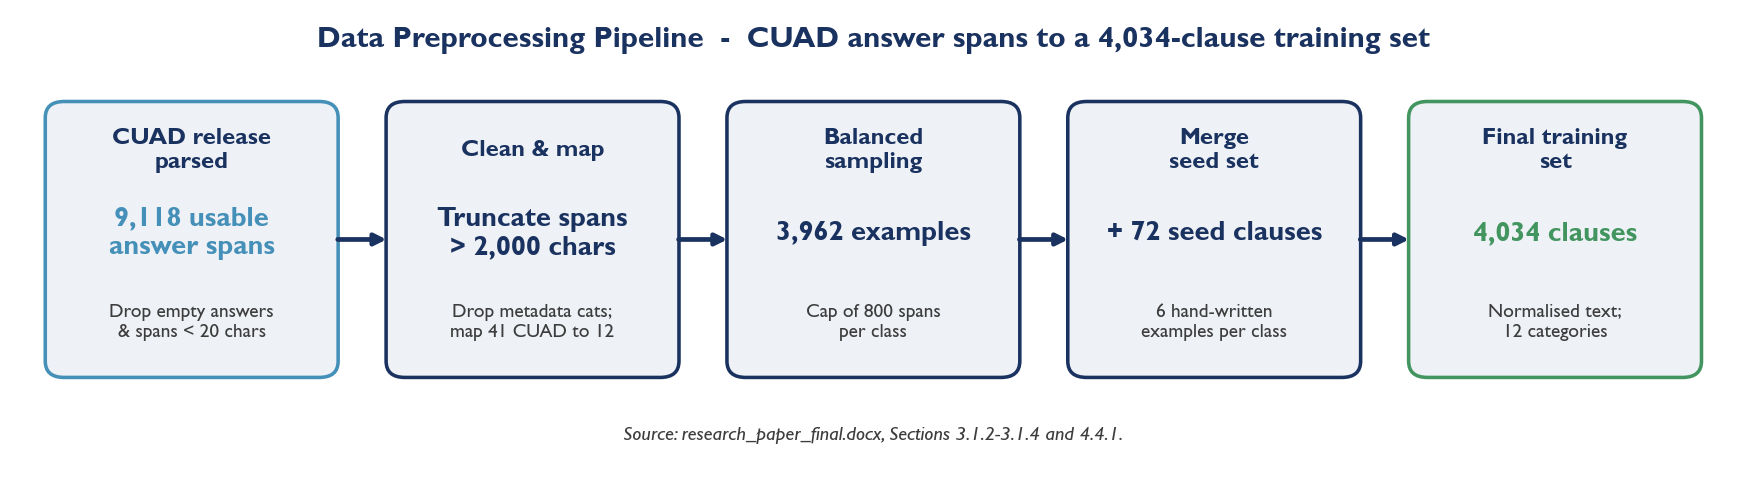
\includegraphics[width=\linewidth]{preprocessing_flow.png}
	\caption{Data preprocessing pipeline: from the raw CUAD release to the 4{,}034-clause training set used by the classifier.}
	\label{fig:preprocessing-flow}
\end{figure}

\begin{figure}[H]
	\centering
	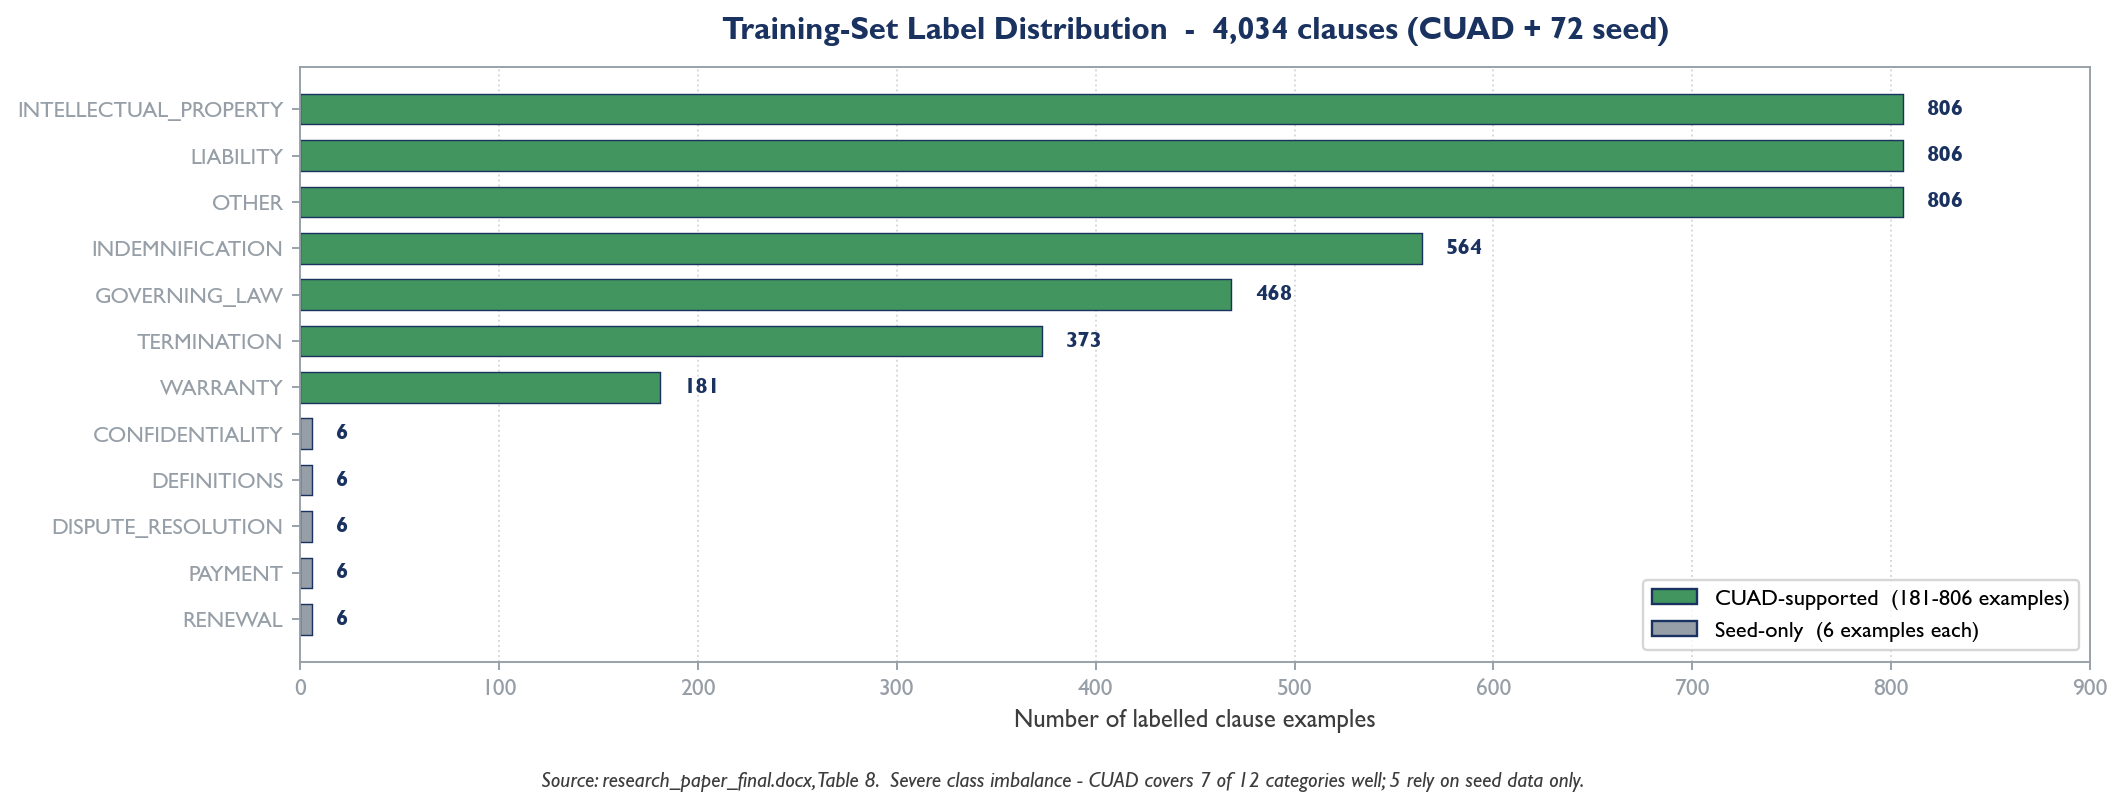
\includegraphics[width=\linewidth]{eda_label_distribution.png}
	\caption{Training-set label distribution across the twelve-category clause taxonomy. Seven categories are well supported by CUAD; five rely on the hand-written seed set.}
	\label{fig:eda-label-distribution}
\end{figure}

\section{System Architecture / Block Diagram / UML Diagram / DFD / Use Case Diagram}

\begin{figure}[H]
	\centering
	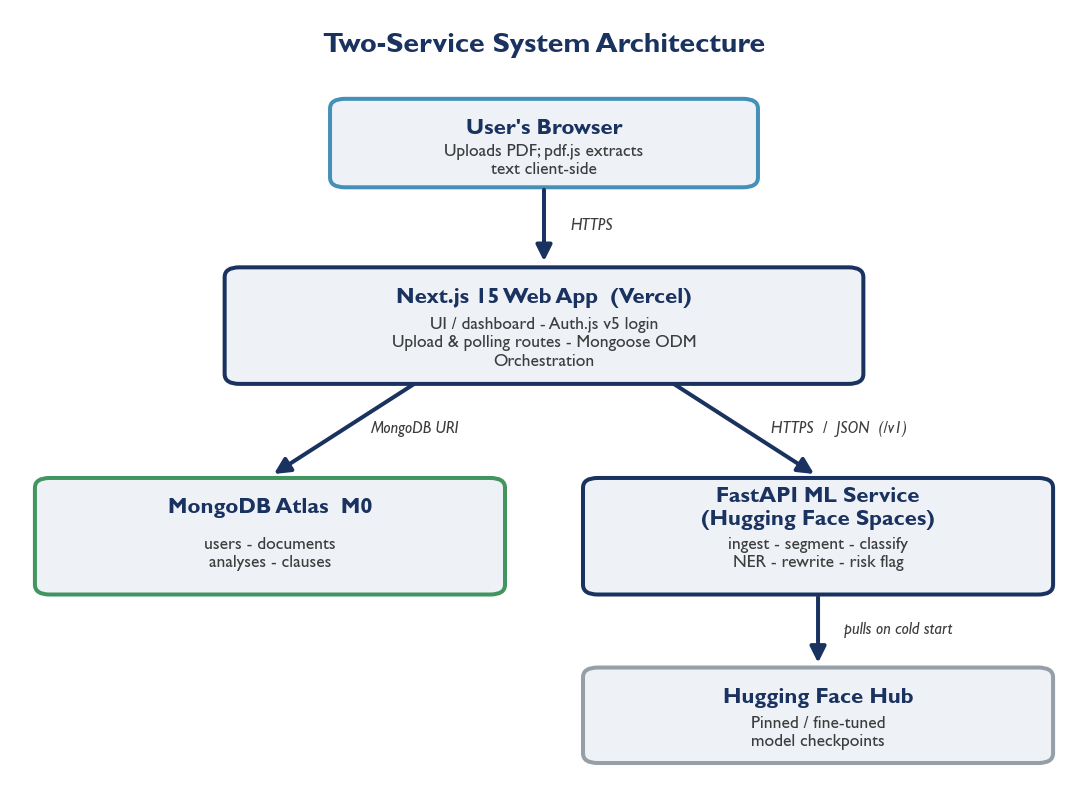
\includegraphics[width=0.78\linewidth]{architecture_diagram.png}
	\caption{Two-service system architecture: a Next.js web application on Vercel handles UI, authentication and persistence; a FastAPI service on Hugging Face Spaces handles all NLP inference.}
	\label{fig:architecture-diagram}
\end{figure}

\section{Methodology / Algorithm / Model Description}

\begin{figure}[H]
	\centering
	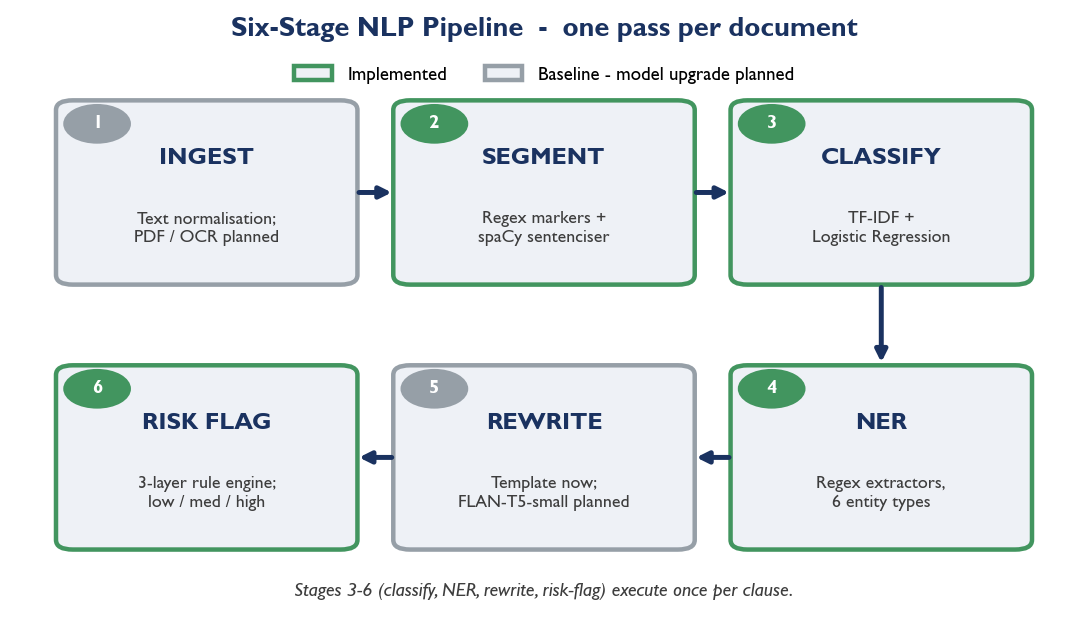
\includegraphics[width=0.95\linewidth]{model_architecture.png}
	\caption{Six-stage NLP pipeline executed by the ML service for every document. Stages 3--6 (classify, NER, rewrite, risk-flag) run once per clause.}
	\label{fig:model-architecture}
\end{figure}

\begin{figure}[H]
	\centering
	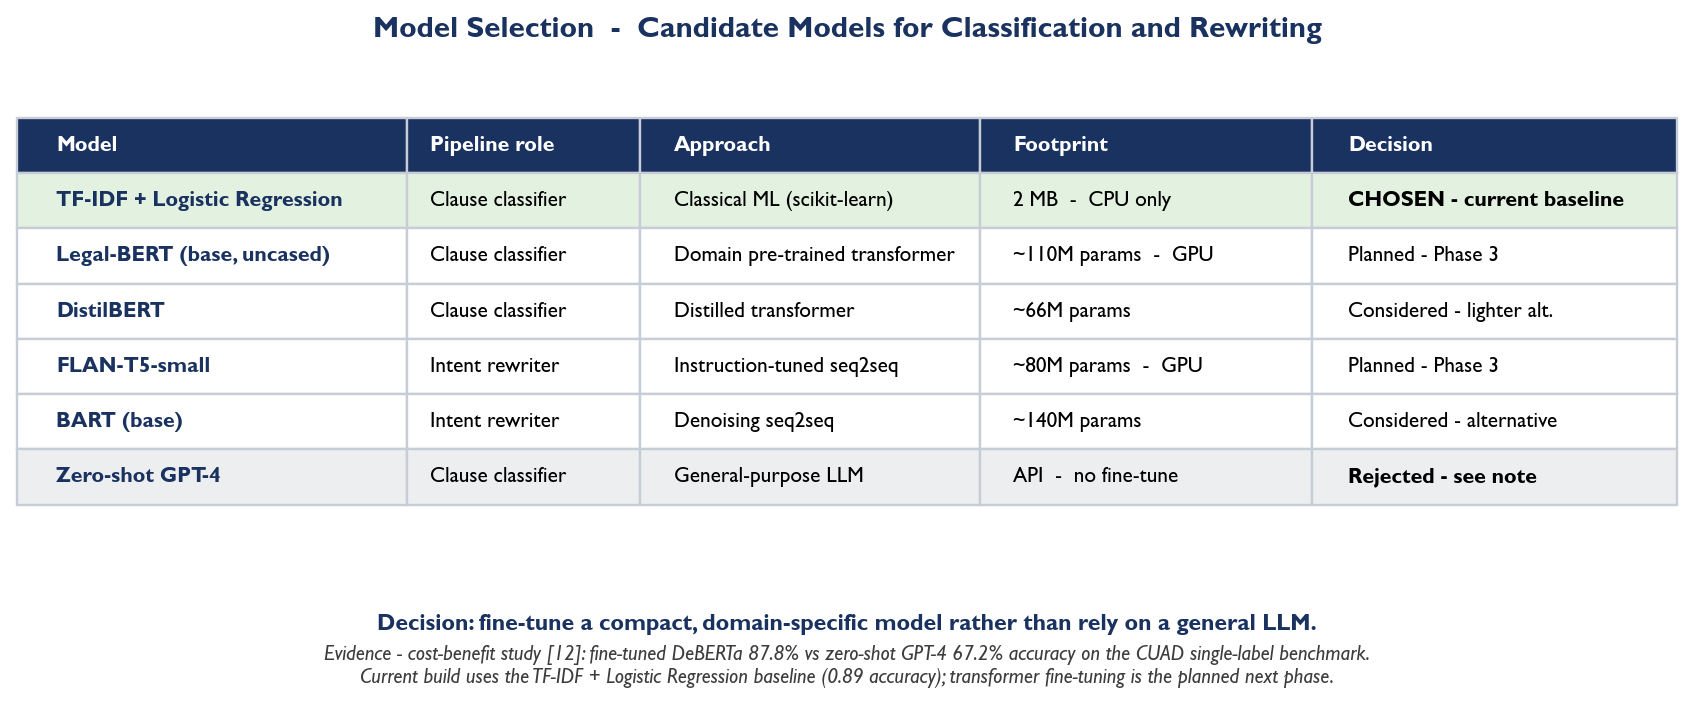
\includegraphics[width=\linewidth]{model_selection.png}
	\caption{Candidate models considered for clause classification and intent rewriting, with the rationale for the chosen TF--IDF baseline (kept as a runtime fallback) and the fine-tuned Legal-BERT and FLAN-T5-small models now deployed in production.}
	\label{fig:model-selection}
\end{figure}

\section{Tools, Technologies and Frameworks Used}
\section{Performance Metrics / Evaluation Criteria}

\begin{figure}[H]
	\centering
	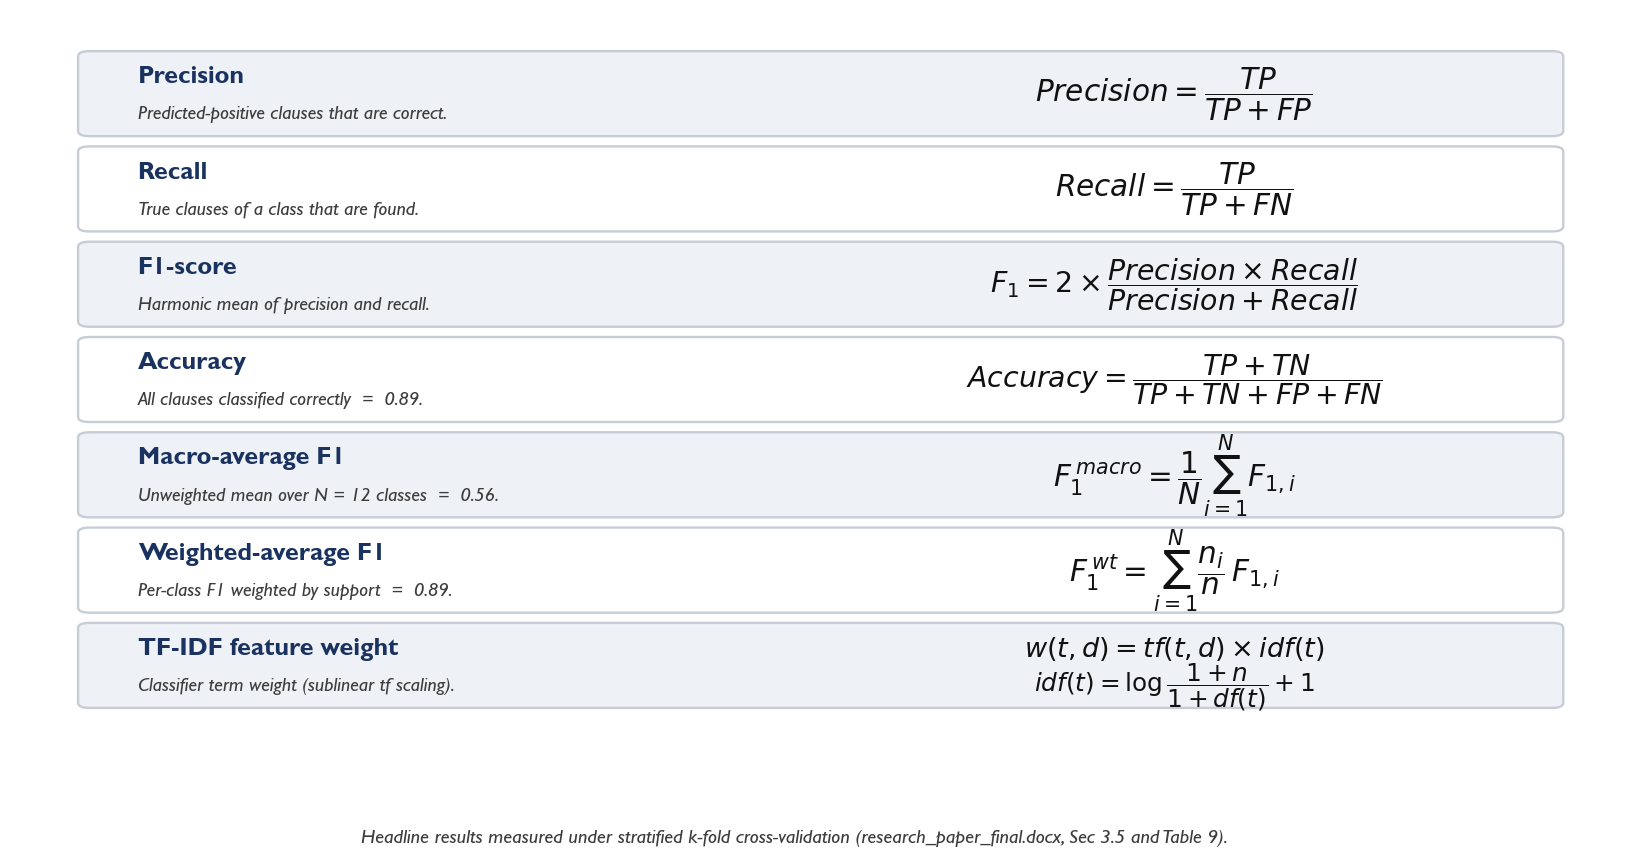
\includegraphics[width=\linewidth]{metrics_formulae.png}
	\caption{Evaluation metrics used in this work: precision, recall, F\textsubscript{1}, accuracy, macro- and weighted-average F\textsubscript{1}, and the TF--IDF feature weighting used by the classifier.}
	\label{fig:metrics-formulae}
\end{figure}


\chapter{EXPERIMENTATION AND RESULTS / APPLICATION/SYSTEM DESIGN AND OUTPUTS }
\section{System Specifications / Experimental Setup}
\section{Parameter Settings / Configuration Details (if applicable)}
\section{Implementation Details / Module Description}
\section{Results and Outputs}

\begin{figure}[H]
	\centering
	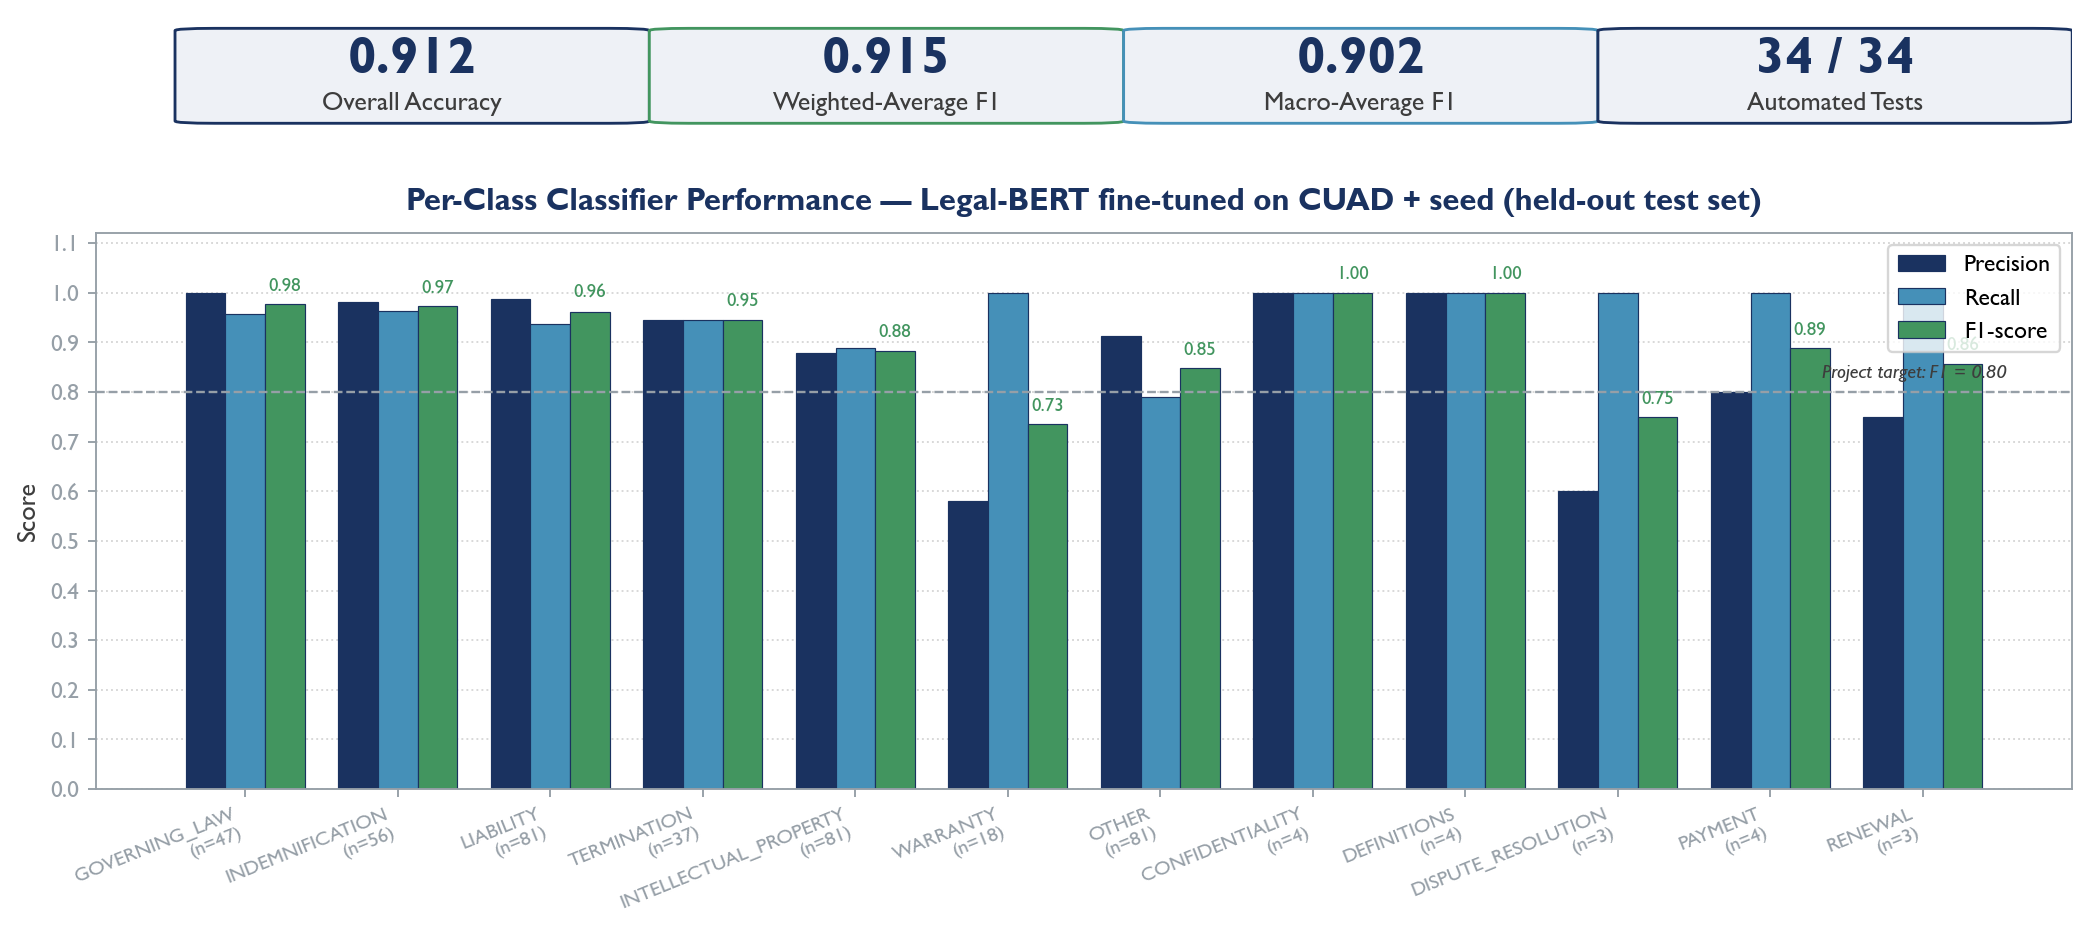
\includegraphics[width=\linewidth]{results_chart.png}
	\caption{Per-class held-out performance of the fine-tuned Legal-BERT classifier (\texttt{freak3123/legal-bert-cuad-v1}). Overall accuracy is 0.912, weighted-average F\textsubscript{1} is 0.915, and macro-average F\textsubscript{1} is 0.902 across all twelve clause categories.}
	\label{fig:results-chart}
\end{figure}

\begin{figure}[H]
	\centering
	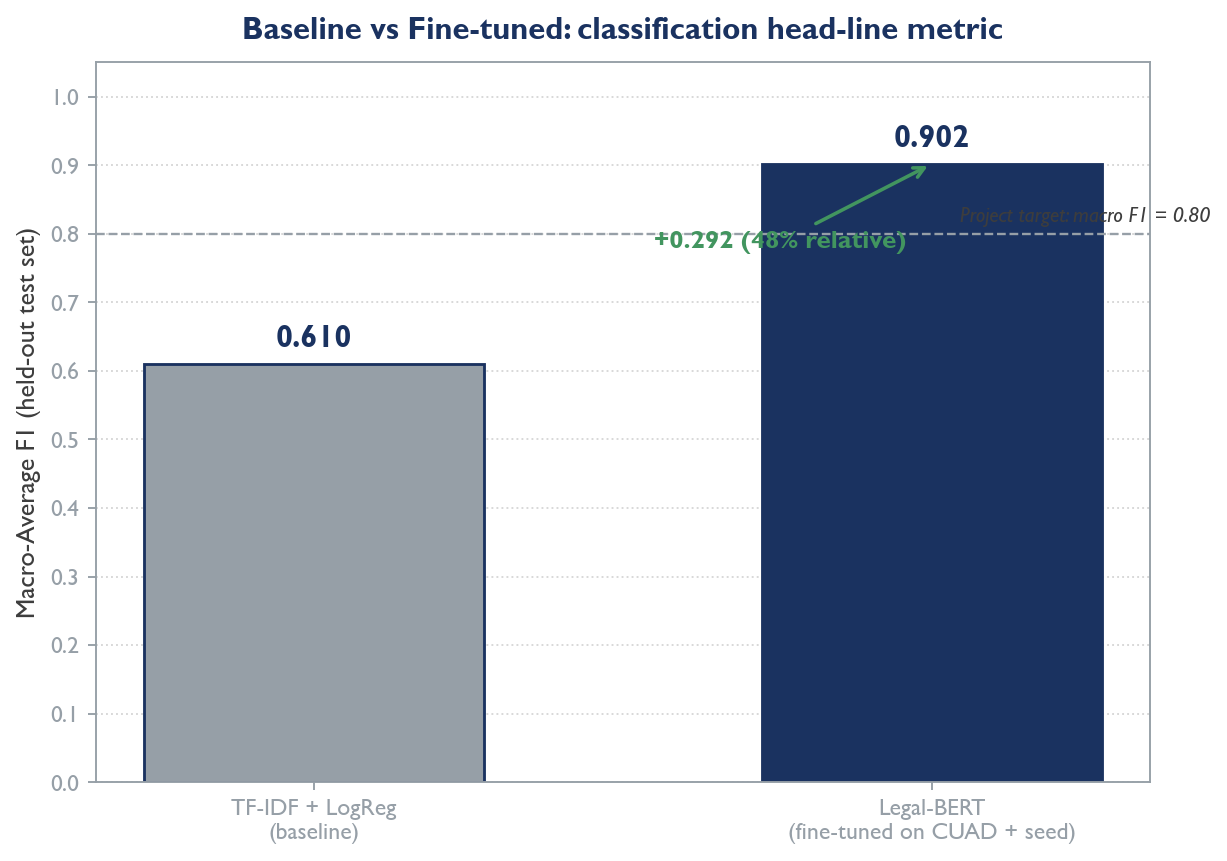
\includegraphics[width=0.7\linewidth]{comparison_baseline_bert.png}
	\caption{Headline metric improvement from baseline to fine-tuned: TF--IDF + Logistic Regression macro F\textsubscript{1} of 0.61 against fine-tuned Legal-BERT macro F\textsubscript{1} of 0.902 on the same held-out 419-clause test set.}
	\label{fig:comparison-baseline-bert}
\end{figure}

\begin{figure}[H]
	\centering
	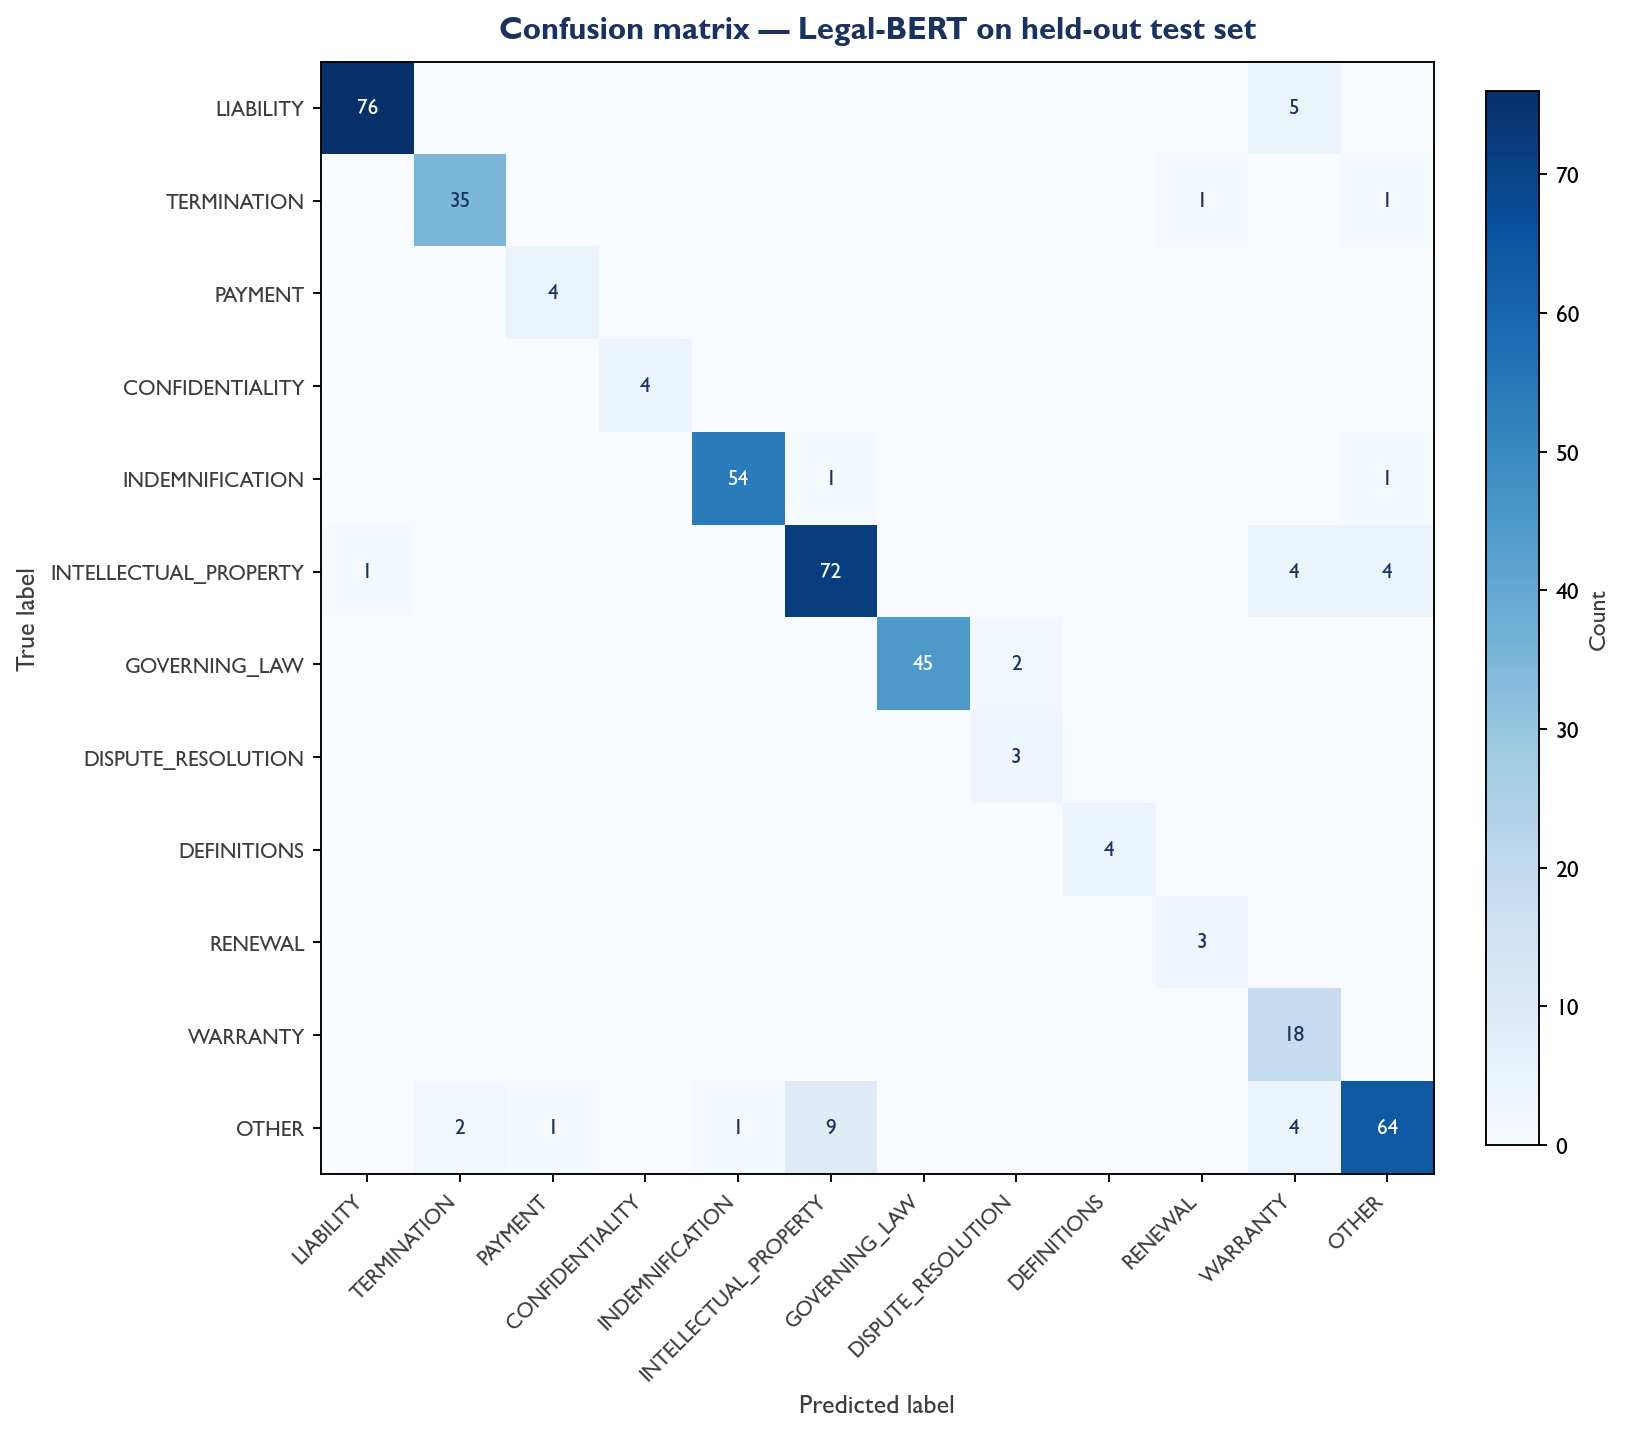
\includegraphics[width=0.85\linewidth]{confusion_matrix.png}
	\caption{Confusion matrix for the fine-tuned Legal-BERT classifier on the held-out 419-clause test set. Off-diagonal mass is concentrated on OTHER $\leftrightarrow$ INTELLECTUAL\_PROPERTY and WARRANTY boundary cases.}
	\label{fig:confusion-matrix}
\end{figure}

\begin{figure}[H]
	\centering
	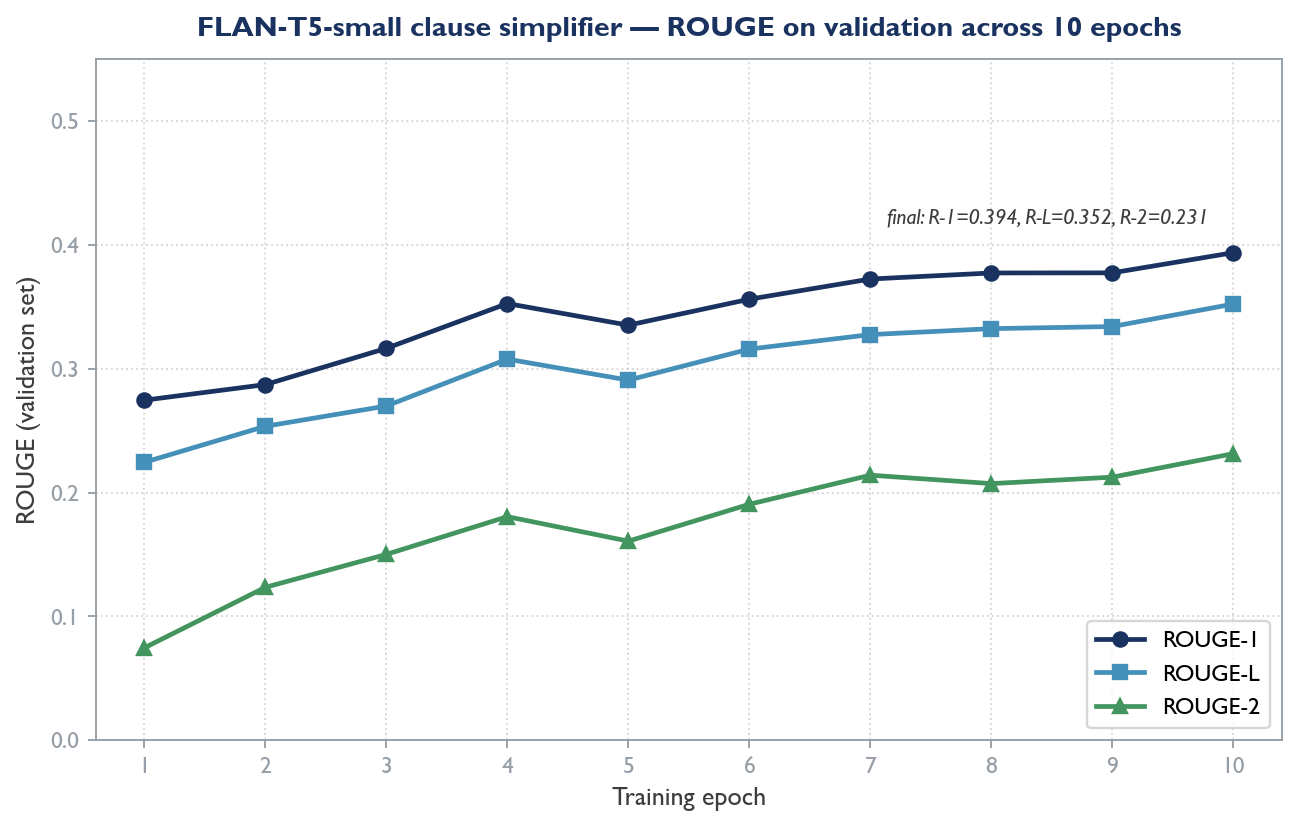
\includegraphics[width=0.85\linewidth]{flan_t5_rouge_curves.png}
	\caption{Validation ROUGE for the fine-tuned FLAN-T5-small clause simplifier (\texttt{freak3123/flan-t5-simplify-v1}) across ten training epochs. Final scores: ROUGE-1 = 0.394, ROUGE-2 = 0.231, ROUGE-L = 0.352.}
	\label{fig:flan-t5-rouge}
\end{figure}

\begin{figure}[H]
	\centering
	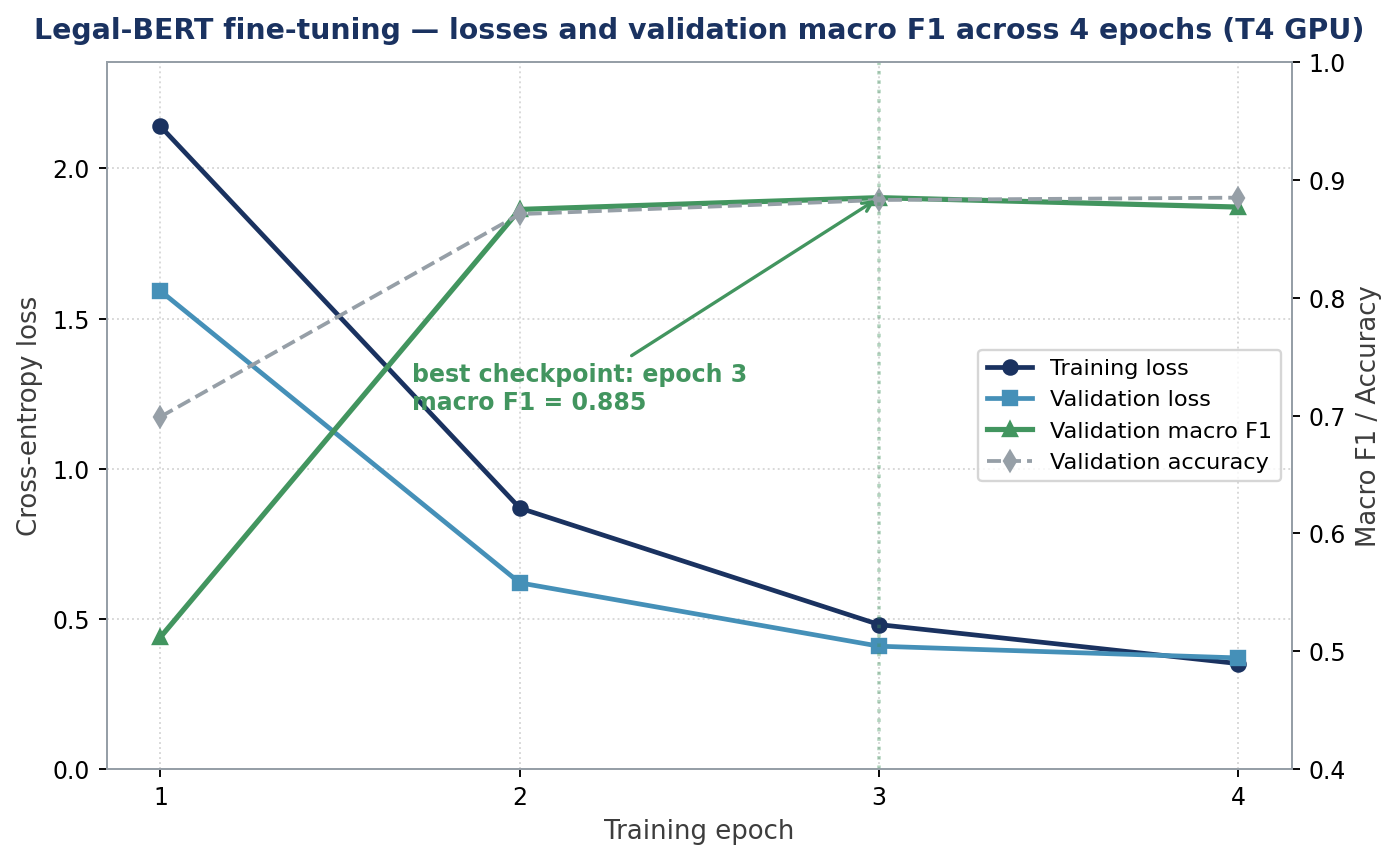
\includegraphics[width=0.85\linewidth]{legal_bert_training_curves.png}
	\caption{Legal-BERT fine-tuning trajectory across the four training epochs on a Kaggle T4 GPU. Training and validation losses fall monotonically while validation macro F\textsubscript{1} climbs from 0.512 at epoch 1 to a best of 0.885 at epoch 3; the trainer saves the epoch-3 checkpoint as the best model.}
	\label{fig:legal-bert-curves}
\end{figure}

\begin{figure}[H]
	\centering
	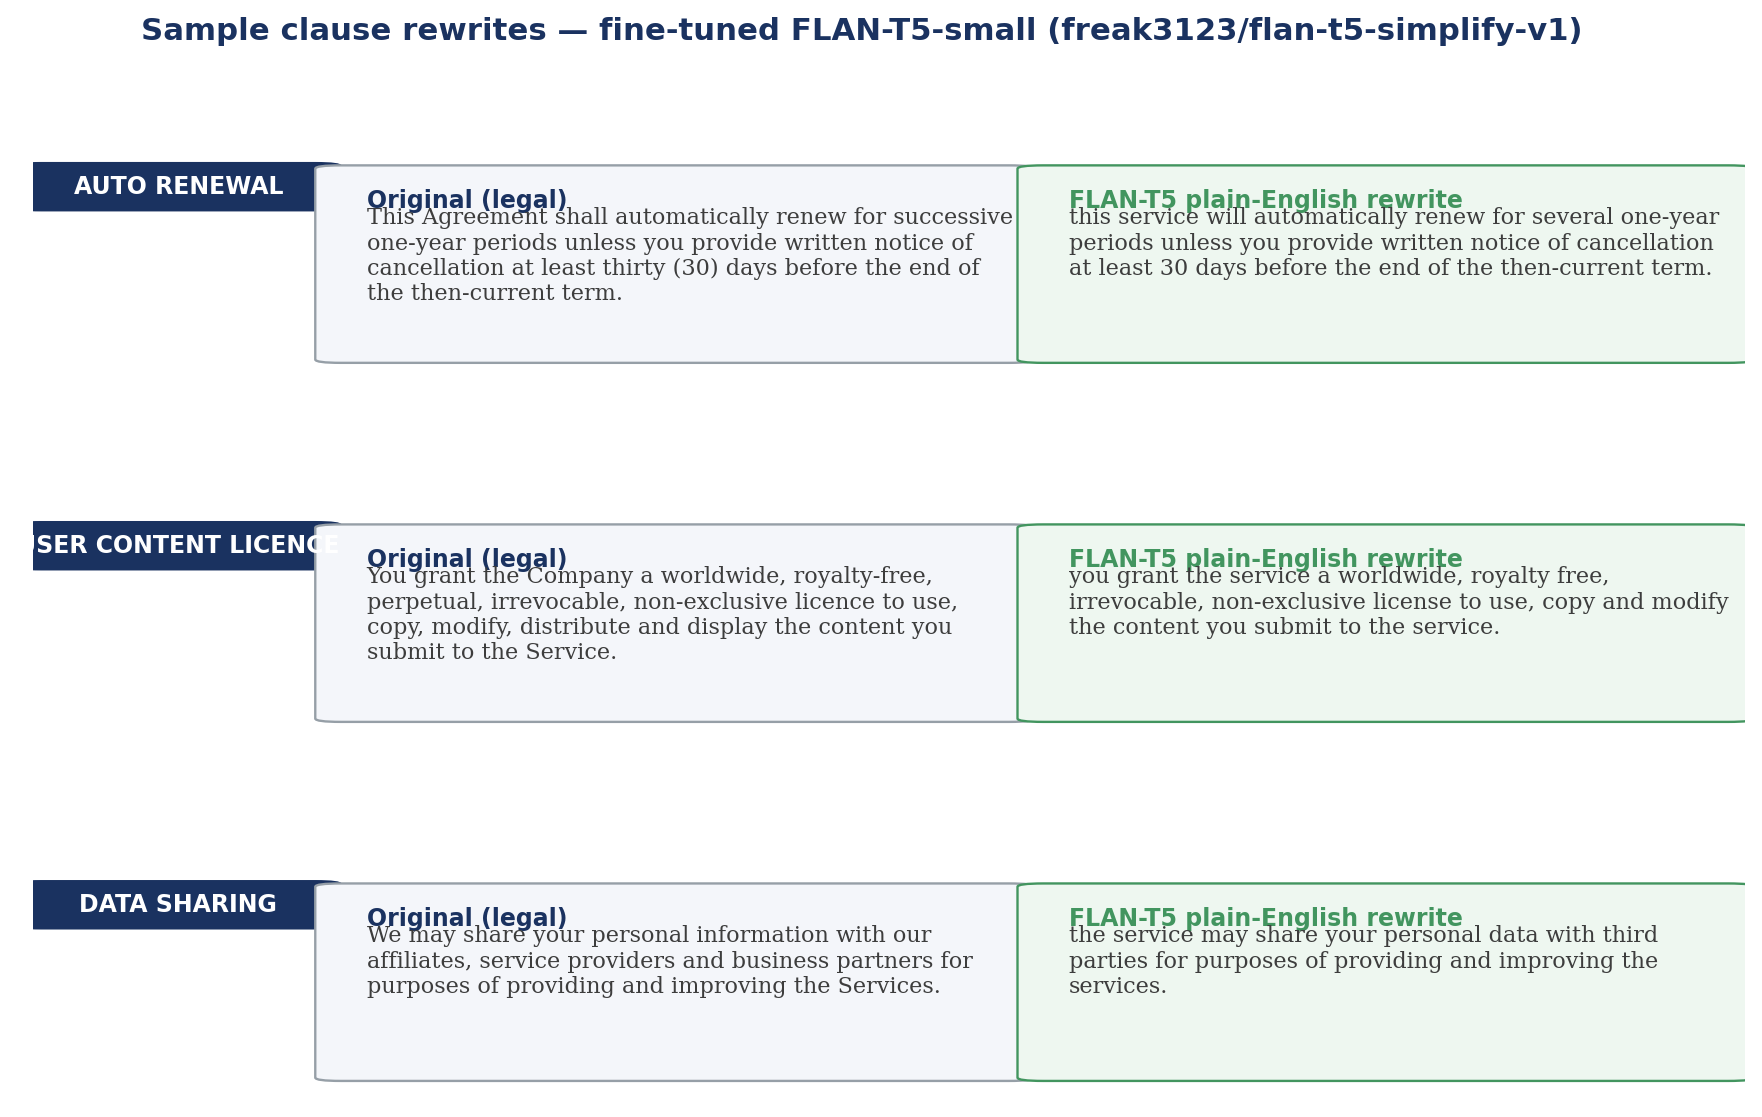
\includegraphics[width=\linewidth]{rewrite_examples.png}
	\caption{Side-by-side legal-to-plain-English rewrites produced by the fine-tuned FLAN-T5-small model on three representative clause types (automatic renewal, user-content licence, data sharing). All outputs are verbatim model generations with no manual editing.}
	\label{fig:rewrite-examples}
\end{figure}

\section{Result Analysis and Validation}

\chapter{ETHICAL, SOCIAL \& SUSTAINABILITY CONSIDERATIONS}
\section{Ethical Consideration}
\section{Social Impact and Societal Relevance}
\section{Sustainability Consideration}


\chapter{CONCLUSION AND FUTURE SCOPES}
\section{Summary of Findings}
\section{Limitations of the Work}
\section{Scope for Future Enhancements}


\chapter*{REFERENCES}
\addcontentsline{toc}{chapter}{REFERENCES}

\begin{enumerate}[label={[{\arabic*}]}]
	\item{} Author(s) (Year), `\textit{Title}', Publisher, Vol.\_\_, Issue \_\_, pp \_\_
    \item{} Author(s) (Year), `\textit{Title}', Publisher, Vol.\_\_, Issue \_\_, pp \_\_
    \item{} Author(s) (Year), `\textit{Title}', Publisher, Vol.\_\_, Issue \_\_, pp \_\_
    \item{} Author(s) (Year), `\textit{Title}', Publisher, Vol.\_\_, Issue \_\_, pp \_\_
\end{enumerate}
	

\chapter*{APPENDIX}
\addcontentsline{toc}{chapter}{APPENDIX}


\section*{Project Proposal}
\addcontentsline{toc}{section}{Project Proposal}


\newpage
\section*{Similarity Check Report}
\addcontentsline{toc}{section}{Similarity Check Report}


\newpage
\section*{Team Contribution}
\addcontentsline{toc}{section}{Team Contribution}

\begin{tabular}{|p{5cm}| p{10cm}|}
\hline
\multicolumn{1}{|c|}{\textbf{Name}} & \multicolumn{1}{|c|}{\textbf{Contribution}}\\ \hline
Student 01 Name & \\ \hline
Student 02 Name & \\ \hline
Student 03 Name & \\ \hline
Student 04 Name & \\ \hline
\end{tabular}


\newpage
\section*{Course Outcomes (COs), Program Outcomes (POs) and Program Specific Outcomes (PSOs)}
\addcontentsline{toc}{section}{Course Outcomes (COs), Program Outcomes (POs) and Program Specific Outcomes (PSOs)}


\subsection*{Course Outcomes (COs)}
\begin{enumerate}[leftmargin=3em]
	\item[\textbf{CO1:}] Apply engineering knowledge and computing fundamentals to analyze complex real-world problems, identify requirements, and define appropriate project objectives.
	\item[\textbf{CO2:}] Design and develop end-to-end software or computing solutions using appropriate algorithms, architectures, and modern tools to meet specified constraints.
	\item[\textbf{CO3:}] Conduct investigations, experimentation, and performance evaluation using suitable metrics, datasets, simulations, or prototypes to validate project outcomes.
	\item[\textbf{CO4:}] Demonstrate the ability to function effectively as an individual and as a team member/leader, managing tasks, timelines, and resources in multidisciplinary environments.
	\item[\textbf{CO5:}] Communicate technical ideas, design decisions, and results effectively through well-structured project reports, presentations, and demonstrations.
	\item[\textbf{CO6:}] Recognize and apply professional ethics, societal impact, sustainability considerations, and lifelong learning principles in project development and execution.
\end{enumerate}



\subsection*{Program Outcomes (POs)}
\begin{enumerate}[leftmargin=3em]
\item[\textbf{PO1:}] \textbf{Engineering knowledge:} Apply the knowledge of mathematics, science, engineering fundamentals and an engineering specialization to the solution of complex engineering problems.

\item[\textbf{PO2:}] \textbf{Problem analysis:} Identify, formulate, review research literature and analyze complex engineering problems reaching substantiated conclusions using first principles of mathematics, natural sciences and engineering sciences.

\item[\textbf{PO3:}] \textbf{Design/development of solutions:} Design solutions for complex engineering problems and design system components or processes that meet specified needs with appropriate consideration for public health and safety, and cultural, societal and environmental considerations.

\item[\textbf{PO4:}] \textbf{Conduct investigations of complex problems:} Use research-based knowledge and research methods including design of experiments, analysis and interpretation of data and synthesis of information to provide valid conclusions.

\item[\textbf{PO5:}] \textbf{Modern tool usage:} Create, select and apply appropriate techniques, resources and modern engineering and IT tools including prediction and modeling to complex engineering activities with an understanding of the limitations.

\item[\textbf{PO6:}] \textbf{The engineer and society:} Apply reasoning informed by contextual knowledge to assess societal, health, safety, legal and cultural issues and the consequent responsibilities relevant to professional engineering practice.

\item[\textbf{PO7:}] \textbf{Environment and sustainability:} Understand the impact of professional engineering solutions in societal and environmental contexts and demonstrate knowledge of, and need for, sustainable development.

\item[\textbf{PO8:}] \textbf{Ethics:} Apply ethical principles and commit to professional ethics and responsibilities and norms of engineering practice.

\item[\textbf{PO9:}] \textbf{Individual and teamwork:} Function effectively as an individual, and as a member or leader in diverse teams and in multidisciplinary settings.

\item[\textbf{PO10:}] \textbf{Communication:} Communicate effectively on complex engineering activities with the engineering community and with society at large.

\item[\textbf{PO11:}] \textbf{Project management and finance:} Demonstrate knowledge and understanding of engineering and management principles and apply these to one’s own work as a member and leader in a team to manage projects in multidisciplinary environments.

\end{enumerate}


\subsection*{Program Specific Outcomes (PSOs)}

\begin{enumerate}[leftmargin=3.25em]
	\item[\textbf{PSO1:}] 	The ability to understand and develop computer programs in the areas related to business intelligence, big data analytics, web design and networking for efficient design of computer-based system of varying complexity.
	\item[\textbf{PSO2:}] The ability to apply standard practices and strategy in software project development using open ended programming environments to deliver a quality product for business success.


\end{enumerate}


\newpage
\section*{Evidences Linked to CO–PO \& PSO Mapping}
\addcontentsline{toc}{section}{Evidences Linked to CO–PO \& PSO Mapping}



\footnotesize

\begin{longtable}{|c|p{3cm}|p{9cm}|p{2.0cm}|}
\hline
\centering\textbf{COs} &
\centering\textbf{Mapped POs and PSOs} &
\multicolumn{2}{c|}{\textbf{Evidence in Project Work}}
\\ \cline{3-4}

& &
\centering\textbf{Description} &
\centering\textbf{Section with Evidence}
\\ %\hline

\endfirsthead

\hline
\centering\textbf{COs} & 
\centering\textbf{Mapped POs and PSOs} & 
\centering\textbf{Description} &
{\centering\textbf{Section with Evidence}} \\
\hline
\endhead

\hline
\multicolumn{4}{r}{\textit{Continued on next page}}\\
\endfoot

\hline
\endlastfoot

\hline
% ---------------- CO1 ----------------
\multirow{3}{*}{\textbf{CO1}}
& {\textbf{PO1}\newline(Engineering Knowledge)}
& 			 1.
	\newline 2. 
	\newline 3. 
& - \newline - \newline - \\ \cline{2-4}

& {\textbf{PO2}\newline(Problem Analysis)}
& 			 1.
	\newline 2. 
	\newline 3. 
& - \newline - \newline - \\ \cline{2-4}

& {\textbf{PSO1}}
& 			 1.
	\newline 2. 
	\newline 3. 
& - \newline - \newline - \\ \hline
% ---------------- CO2 ----------------
\multirow{3}{*}{\textbf{CO2}}
& {\textbf{PO3}\newline(Design/Development of Solutions)}
& 		 	 1.
	\newline 2. 
	\newline 3. 

&  - \newline - \newline - \\ \cline{2-4}

& {\textbf{PO5}\newline(Engineering Tool Usage)}
& 		 	 1.
	\newline 2. 
	\newline 3. 
& - \newline - \newline - \\ \cline{2-4}

& {\textbf{PSO1}}
& 			 1.
	\newline 2. 
	\newline 3. 
& - \newline - \newline - \\ \hline
% ---------------- CO3 ----------------
\multirow{5}{*}{\textbf{CO3}}
& {\textbf{PO2}\newline(Problem Analysis)}
& 		 	 1.
	\newline 2. 
	\newline 3. 
&  - \newline - \newline - \\ \cline{2-4}

& {\textbf{PO4}\newline(Investigation of Complex Problems)}
& 	 	 	 1.
	\newline 2. 
	\newline 3. 
& - \newline - \newline - \\ \cline{2-4}

& {\textbf{PO4}\newline(Investigation of Complex Problems)}
& 	 	 	 1.
	\newline 2. 
	\newline 3. 
& - \newline - \newline - \\ \cline{2-4}

& {\textbf{PSO1}}
& 			 1.
	\newline 2. 
	\newline 3. 
& - \newline - \newline - \\ \cline{2-4}

& {\textbf{PSO2}}
& 			 1.
	\newline 2. 
	\newline 3. 
& - \newline - \newline - \\ \hline

% ---------------- CO4 ----------------
\multirow{3}{*}{\textbf{CO4}}
& {\textbf{PO8}\newline(Individual \& Collaborative Team Work)}
& 		 	 1.
	\newline 2. 
	\newline 3. 
&    - \newline - \\ \cline{2-4}

& {\textbf{PO10}\newline(Project Management \& Finance)}
& 		 	 1.
	\newline 2. 
	\newline 3. 
& - \newline - \newline - \\ \cline{2-4}

& {\textbf{PSO2}}
& 			 1.
	\newline 2. 
	\newline 3. 
& - \newline - \newline - \\ \hline

% ---------------- CO5 ----------------
\textbf{CO5}
& {\textbf{PO9}\newline(Communication)}
& 		 	 1.
	\newline 2. 
	\newline 3. 
& - \newline - \newline - \\ \hline

% ---------------- CO6 ----------------
\multirow{3}{*}{\textbf{CO6}}
& {\textbf{PO6}\newline(The Engineer and the World)}
& 		  	 1.
	\newline 2. 
	\newline 3. 
& - \newline - \newline -\\ \cline{2-4}

& {\textbf{PO7}\newline(Ethics)}
& 		 	 1.
	\newline 2. 
	\newline 3. 
& - \newline - \newline - \\ \cline{2-4}

& {\textbf{PO11}\newline(Life-Long Learning)}
& 		 	 1.
	\newline 2. 
	\newline 3. 
& - \newline - \newline - \\ \hline

\end{longtable}


\newpage
\section*{Code Structure}
\addcontentsline{toc}{section}{Code Structure}



\newpage
\section*{Code Listings}
\addcontentsline{toc}{section}{Code Listings}


\end{document}